\chapter{Klasifiasi Teks}
\section{Jesron Marudut Hatuan/1164077}

\subsection{Teori}
\begin{enumerate}
\item Pengertian Klasifikasi teks
\par Klasifikasi merupakan sebuah kata serapan yang berasal dari bahasa Belanda, yaitu classificatie, yang sendirinya berasal dari bahasa Prancis classification. Istilah ini menunjuk pada metode untuk menyusun data secara sistematis atau menurut beberapa aturan atau kaidah yang telah ditetapkan.
Di dalam kamus besar bahasa Indonesia, klasifikasi adalah penyusunan bersistem dalam kelompok atau golongan menurut kaidah atau standar yang ditetapkan. Secara harafiah bisa pula dikatakan bahwa klasifikasi adalah pembagian sesuatu menurut kelas-kelas. Menurut Ilmu Pengetahuan, Klasifikasi adalah Proses pengelompokkan benda berdasarkan ciri-ciri dari persamaan dan perbedaan.
\begin{figure}[ht]
\centering
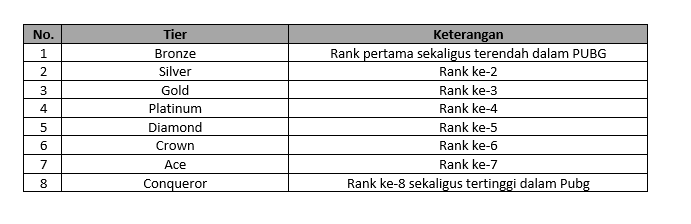
\includegraphics[scale=0.5]{figures/ch4/1.png}
\caption{Klasifikasi teks}
\label{Ilustrasi Klasifikasi Teks}
\end{figure}
	
\item Alasan Klasfikasii Bunga tidak bisa menggunakan machine learning
\par Machine Learning tidak dapat mengklasifikasikan bunga, dikarena data yang diberikan pada  mesin itu akan di algoritmakan untuk mencari sesuatu yang menarik dalam data yang kita berikan, hingga akhirnya sistem AI akan membangun pengetahuan berdasarkan data tersebut. Dengan maksud pembelajaran mesin data beradaptasi terhadap suatu masalah dengan mempelajari pola-pola yang ditemukan dalam data. Sebagai contoh data pada spesies bunga dari genus Iris dengan melihat ukuran sepal (kelopak) dan mahkota pada algoritma data bunga tersebut akan melatih proses pembelajaran pada mesin dalam menganalisa spesies bunga Iris. Dan algoritma pembelajaran mesin akan mempelajari karakteristik dari masing-masing spesies bunga Iris berdasarkan ukuran sepal dan petal yang diberikan.
\begin{figure}[ht]
\centering
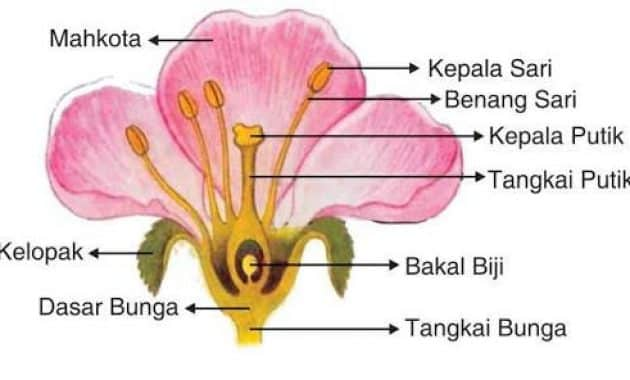
\includegraphics[scale=0.5]{figures/ch4/2.jpg}
\caption{Klasifikasi bunga}
\label{Ilustrasi Klasifikasi Bunga}
\end{figure}

\item
Youtube memungkinkan agar mendapatkan video yang direkomendasikan, karena Machine Learning pada Youtube pasti akan melibatkan data yang sering di lihat oleh penggunanya. Youtube juga akan memberitahukan si pengguna apabila ada video baru yang telah di upload pada chanel yang direkomendasikan untuk si pengguna. Dan apabila menonton video pada youtube maka youtube dapat mengingat dan menggunakan kata tersebut sebagai referensi.

\item Vectorisasi Data
\begin{itemize}
\item proses vektorisasi ini menghasilkan suatu wujud peta yang menggambarkan keadaan permukaan bumi atau bentang alam. Sifat data yang geometris menunjukkan ukuran dimensi yang sesungguhnya.
\end{itemize}
	
\item Bag of word
\par Bag of word merupakan konsep yang diambil dari analisis, kemudian merepresentasikan dokumen berupa kumpulan informasi penting tanpa mengurutkan setiap katanya.
\begin{figure}[ht]
\centering
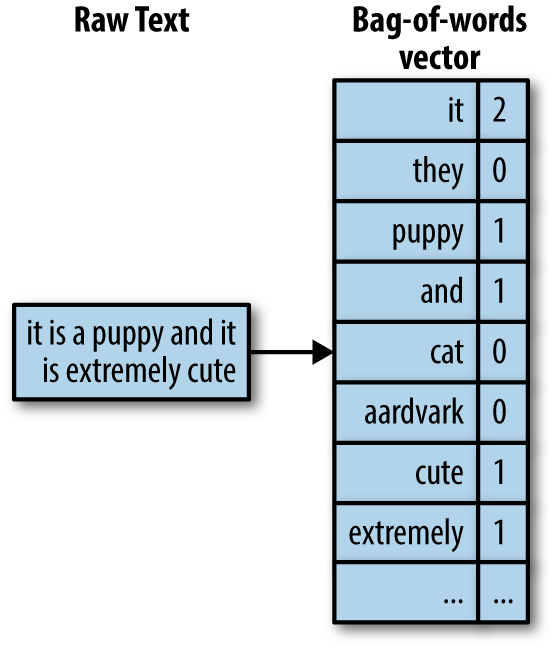
\includegraphics[scale=0.5]{figures/ch4/5.png}
\caption{Bag of Word}
\label{Contoh Ilustrasi}
\end{figure}
	
\item TF-IDF
\par TF-IDF dimaksudkan untuk mencerminkan seberapa relevan suatu istilah dalam dokumen yang diberikan. Intuisi di baliknya adalah bahwa jika sebuah kata muncul beberapa kali dalam sebuah dokumen, kita harus meningkatkan relevansinya karena itu harus lebih bermakna daripada kata-kata lain yang muncul lebih sedikit kali (TF). Pada saat yang sama, jika sebuah kata muncul berkali-kali dalam suatu dokumen tetapi juga di sepanjang banyak dokumen lain, mungkin itu karena kata ini hanya kata yang sering; bukan karena itu relevan atau bermakna (IDF).
\begin{figure}[ht]
\centering
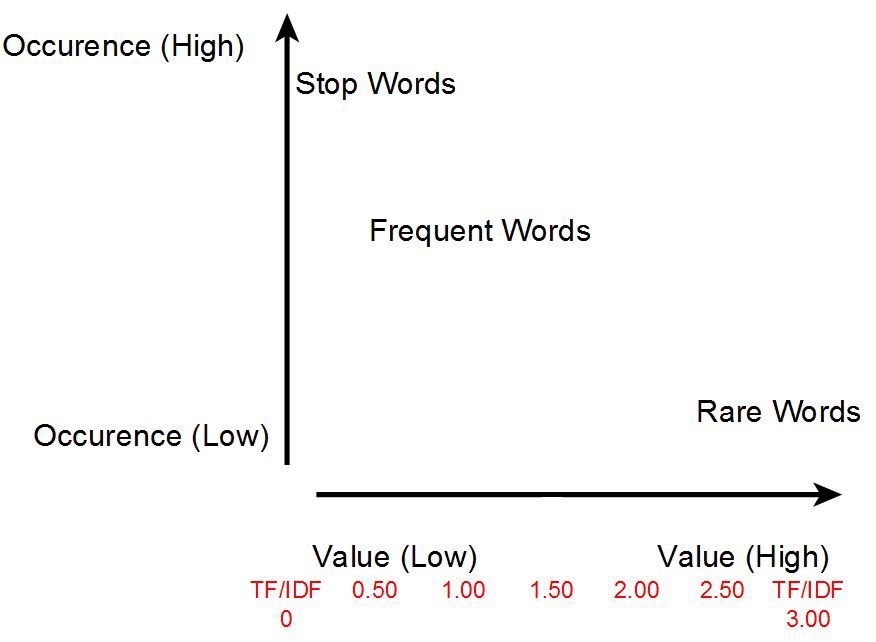
\includegraphics[scale=0.5]{figures/ch4/6.jpeg}
\caption{TF-IDF}
\label{Contoh Ilustrasi}
\end{figure}
\end{enumerate}
